\chapter*{Badania}

Celem tego rozdziału jest przeprowadzenie analizy wyników klasyfikacji obrazów zwierząt dla modeli ResNet i 
ConvNeXt. Analiza obejmuje porównanie skuteczności modeli w różnych scenariuszach modyfikacji tła oraz w zależności 
od wielkości obiektu na obrazie. Przeanalizowane zostaną ogólne metryki, wyniki dla poszczególnych klas oraz wpływ 
wielkości obiektu na dokładność klasyfikacji.


\begin{table}
	\centering
	\begin{tabular}{|c|c|c|c|c|c|}
		\hline
		\textbf{Model} & \textbf{Type} & \textbf{Accuracy} & \textbf{Precision} & \textbf{Recall} & \textbf{F1-score} \\
		\hline
		ResNet & Original & 0.886500 & 0.967026 & 0.886500 & 0.922742 \\
		\hline
		ResNet & Modified & 0.697018 & 0.948539 & 0.697018 & 0.802350 \\
		\hline
		ConvNeXt & Original & 0.943300 & 0.972519 & 0.943300 & 0.956791 \\
		\hline
		ConvNeXt & Modified & 0.790873 & 0.961080 & 0.790873 & 0.866282 \\
		\hline
	\end{tabular}
	\caption{Metryki porównawcze modeli ResNet i ConvNeXt}
	\label{tab:model_comparison_metrics}
\end{table}

\begin{figure}
	\centering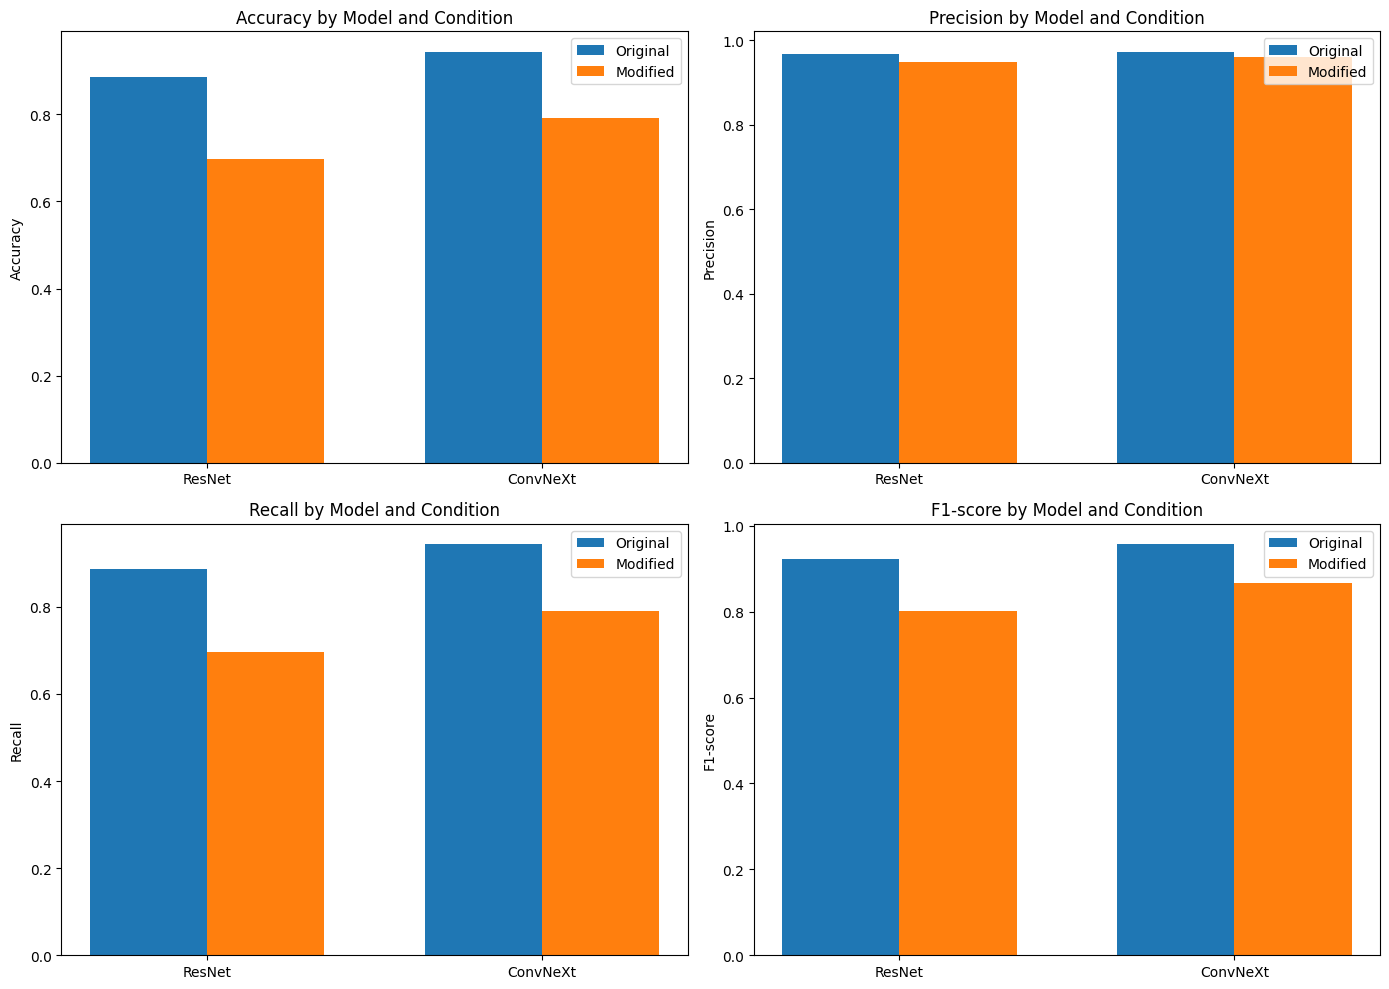
\includegraphics[width=.9\textwidth]{img/overall_metrics}
	\caption{Metryki dla danych oryginalnych zestawionych z danymi o zmodyfikowanych tłach}  
    \label{rys:overall_metrics}
\end{figure}

\begin{table}
	\centering
	\begin{tabular}{|c|c|c|c|c|c|}
		\hline
		\textbf{Model} & \textbf{Type} & \textbf{Average} & 
		\textbf{Average correct} & \textbf{Average incorrect} \\
		\hline
		ResNet & Original & 85.188854 & 89.137424 & 54.348263 \\
		\hline
		ResNet & Modified & 71.694490 & 83.929904 & 43.546579  \\
		\hline
		ConvNeXt & Original & 85.188854 & 89.137424 & 54.348263 \\
		\hline
		ConvNeXt & Modified & 71.694490 & 83.929904 & 43.546579 \\
		\hline
	\end{tabular}
	\caption{Confidence scores dla modeli ResNet i ConvNeXt}
	\label{tab:model_confidence}
\end{table}

\begin{figure}
	\centering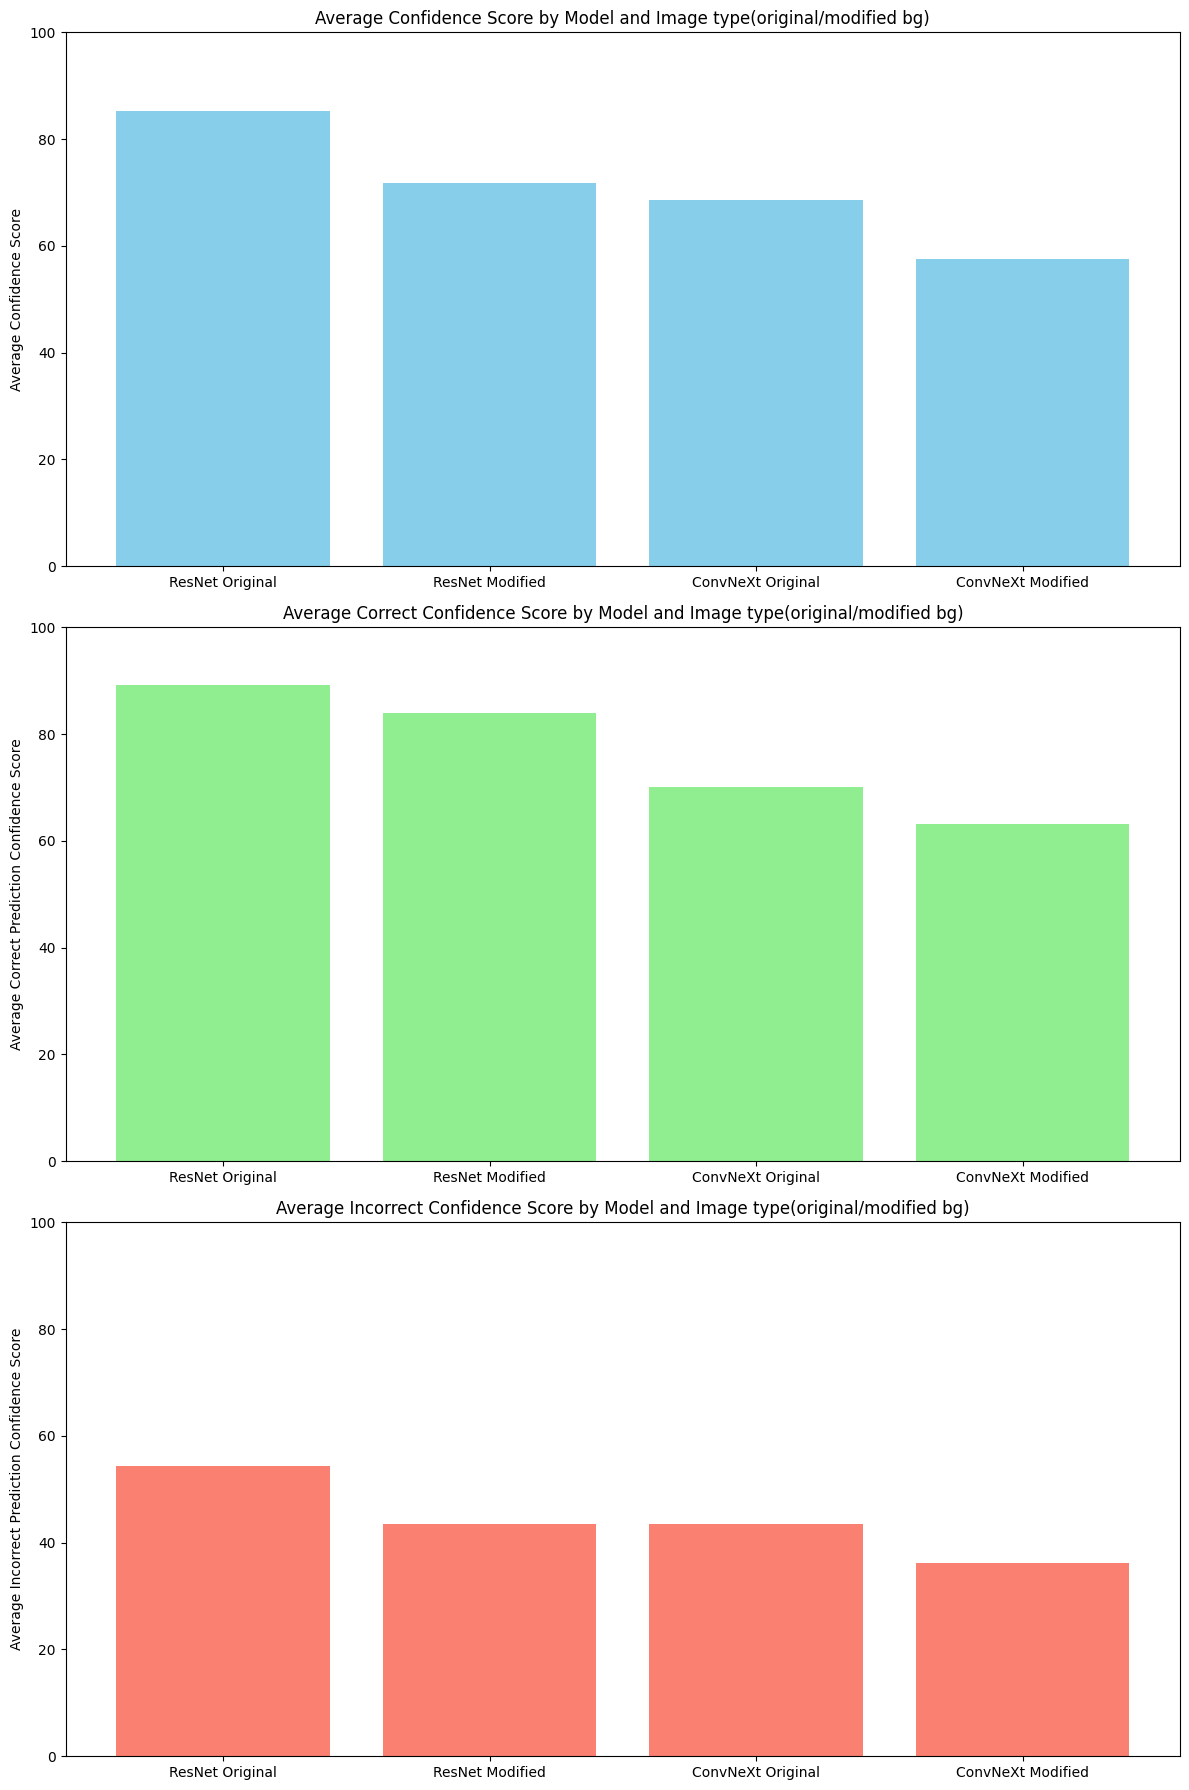
\includegraphics[width=.9\textwidth]{img/confidence_avg}
	\caption{Średnie wartości dla confidence scores}  
    \label{rys:confidence_avg}
\end{figure}

\begin{figure}
	\centering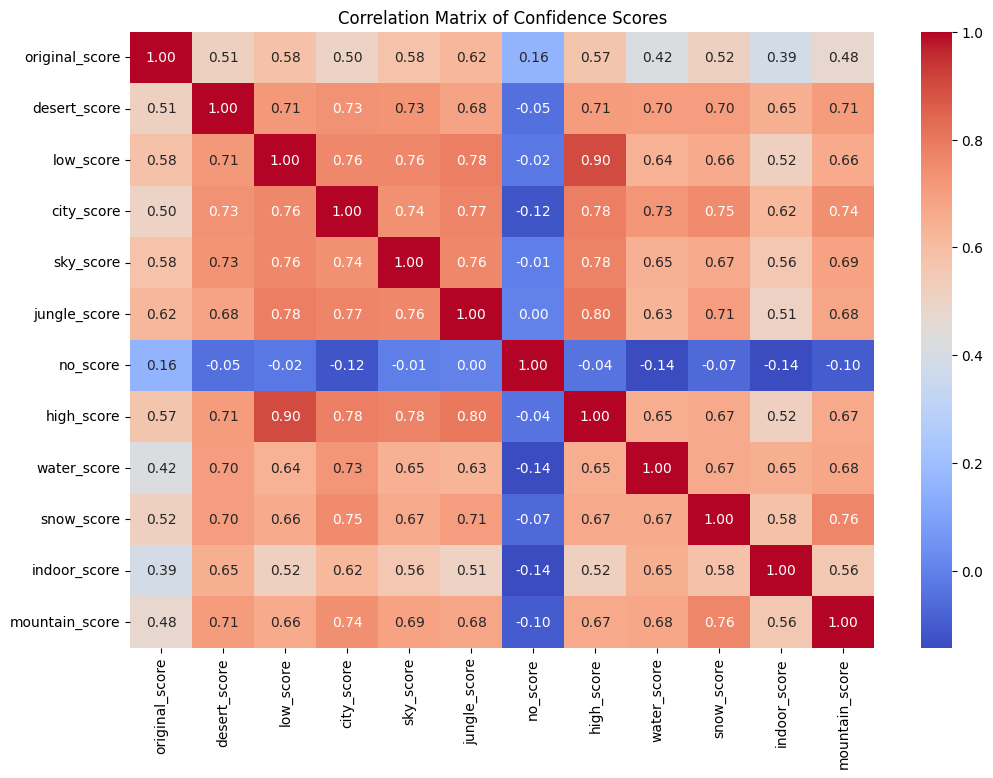
\includegraphics[width=.9\textwidth]{img/correlation_matrix_res}
	\caption{Correlation matrix ResNet confidence}  
    \label{rys:correlation_resnet}
\end{figure}

\begin{figure}
	\centering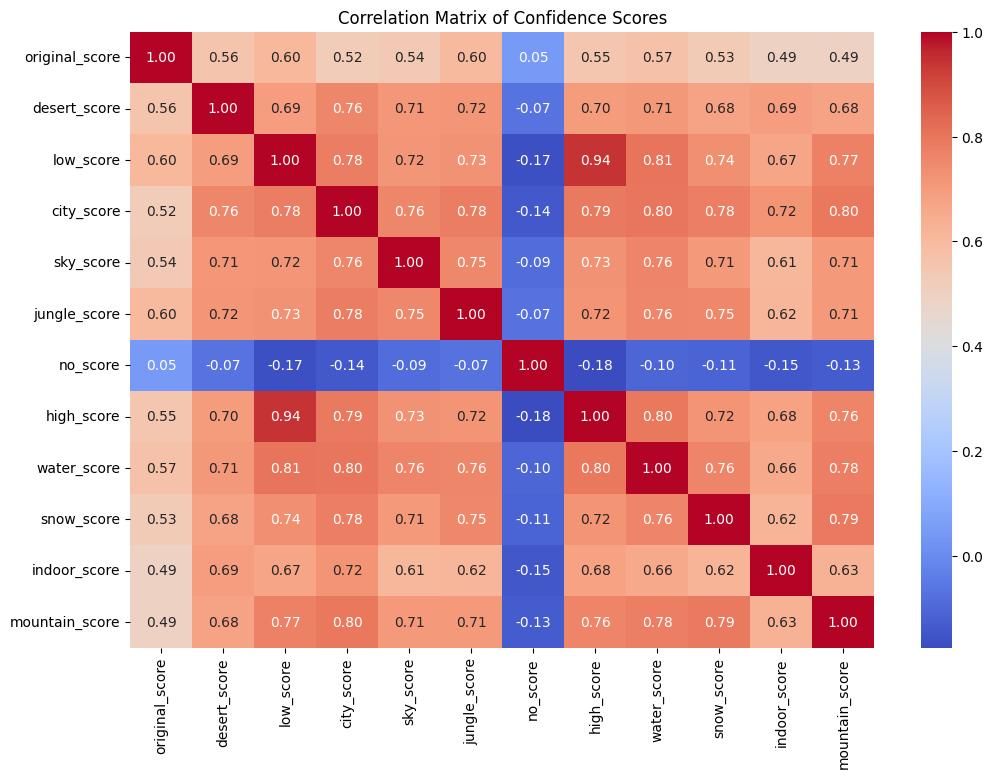
\includegraphics[width=.9\textwidth]{img/correlation_matrix_conv}
	\caption{Correlation matrix ConvNeXt confidence}  
    \label{rys:correlation_convnext}
\end{figure}

\begin{figure}
	\centering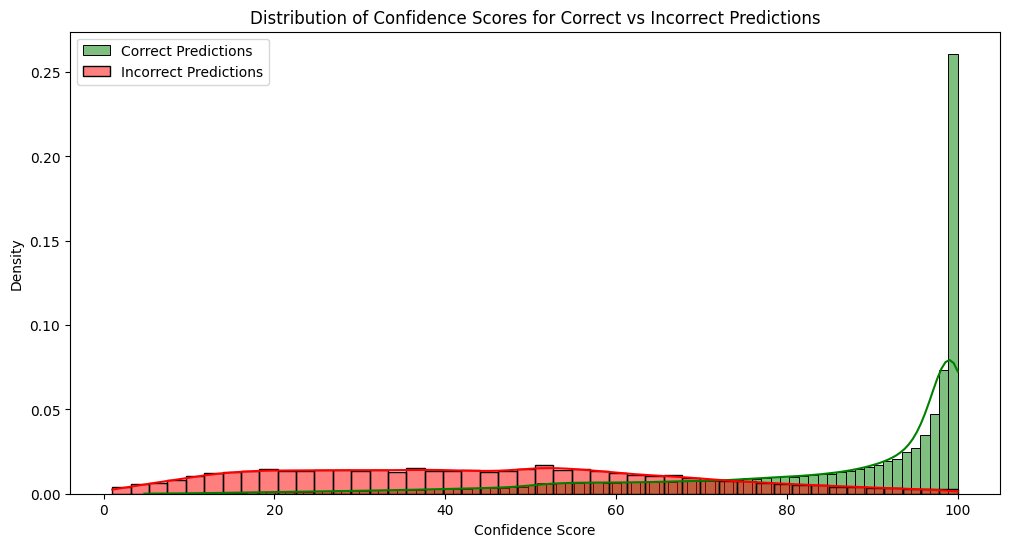
\includegraphics[width=.9\textwidth]{img/resnet_conf_distro}
	\caption{Dystrybucja confidence score dla ResNet}
	\label{rys:res_c_distro}
\end{figure}

\begin{figure}
	\centering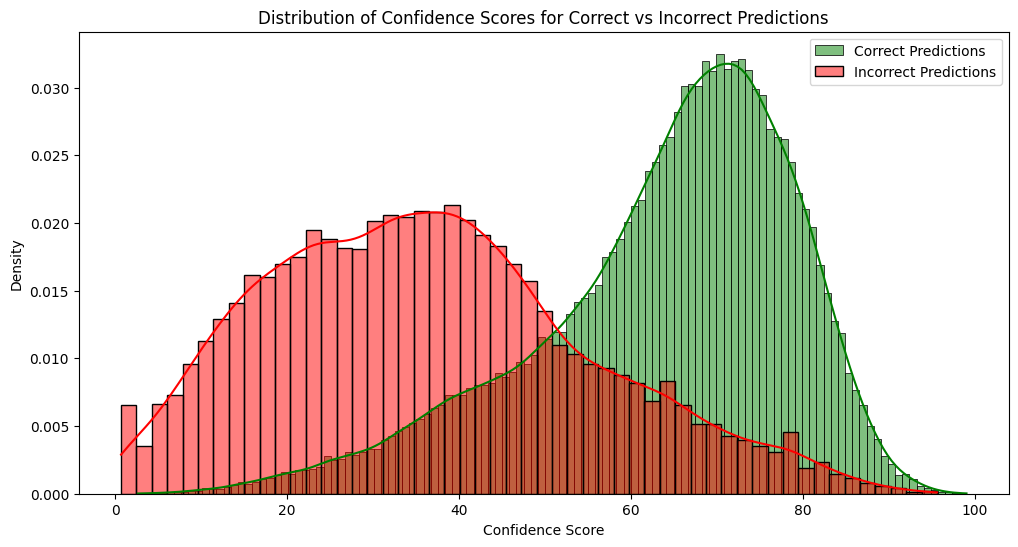
\includegraphics[width=.9\textwidth]{img/convnext_conf_distro}
	\caption{Dystrybucja confidence score dla ConvNext}
	\label{rys:conv_c_distro}
\end{figure}

\begin{figure}
	\centering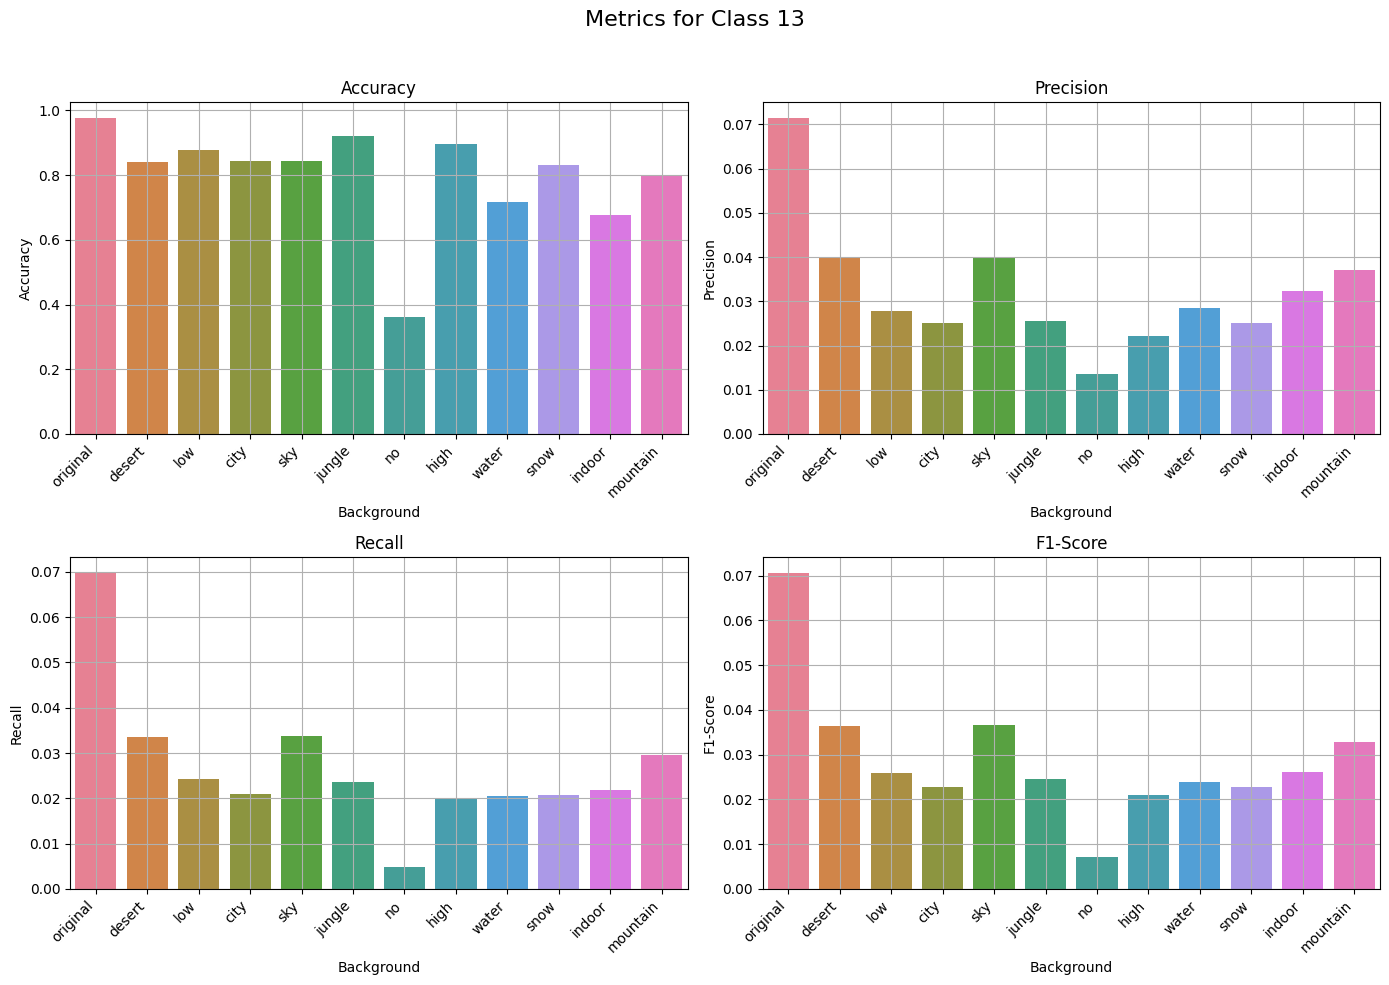
\includegraphics[width=.9\textwidth]{img/13}
	\caption{Metryki}
	\label{rys:13}
\end{figure}

\begin{figure}
	\centering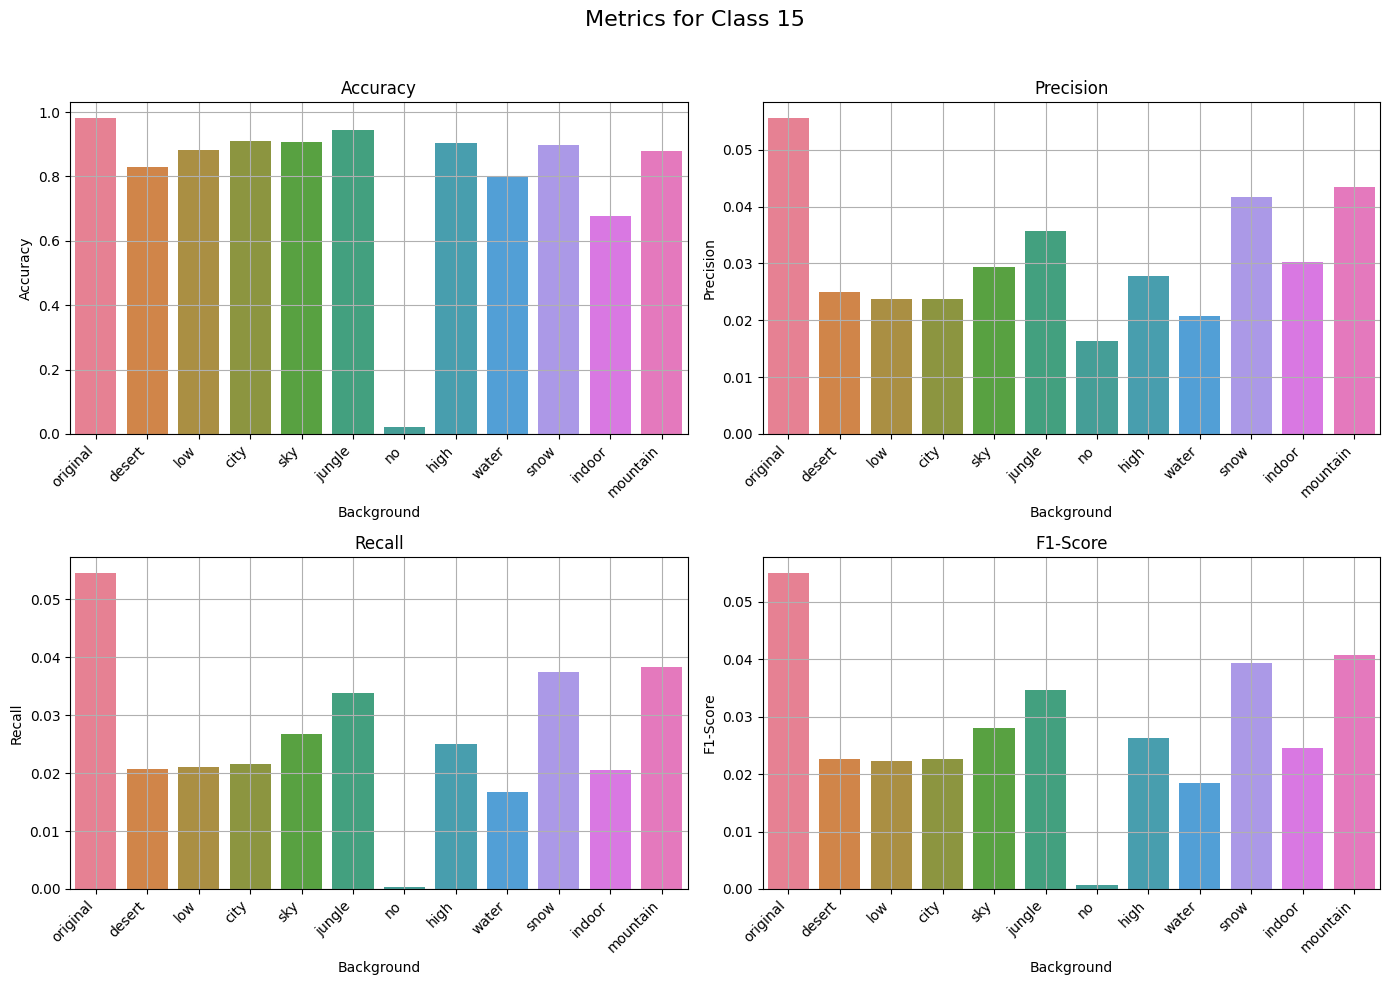
\includegraphics[width=.9\textwidth]{img/15}
	\caption{Metryki}
	\label{rys:15}
\end{figure}

\begin{figure}
	\centering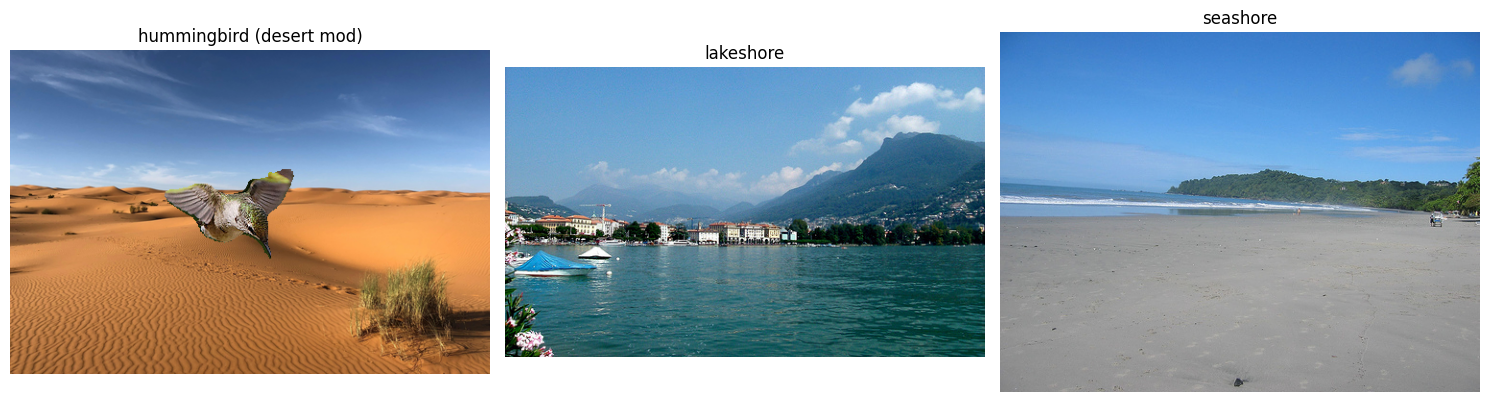
\includegraphics[width=.9\textwidth]{img/94}
	\caption{Metryki}
	\label{rys:94}
\end{figure}

\begin{figure}
	\centering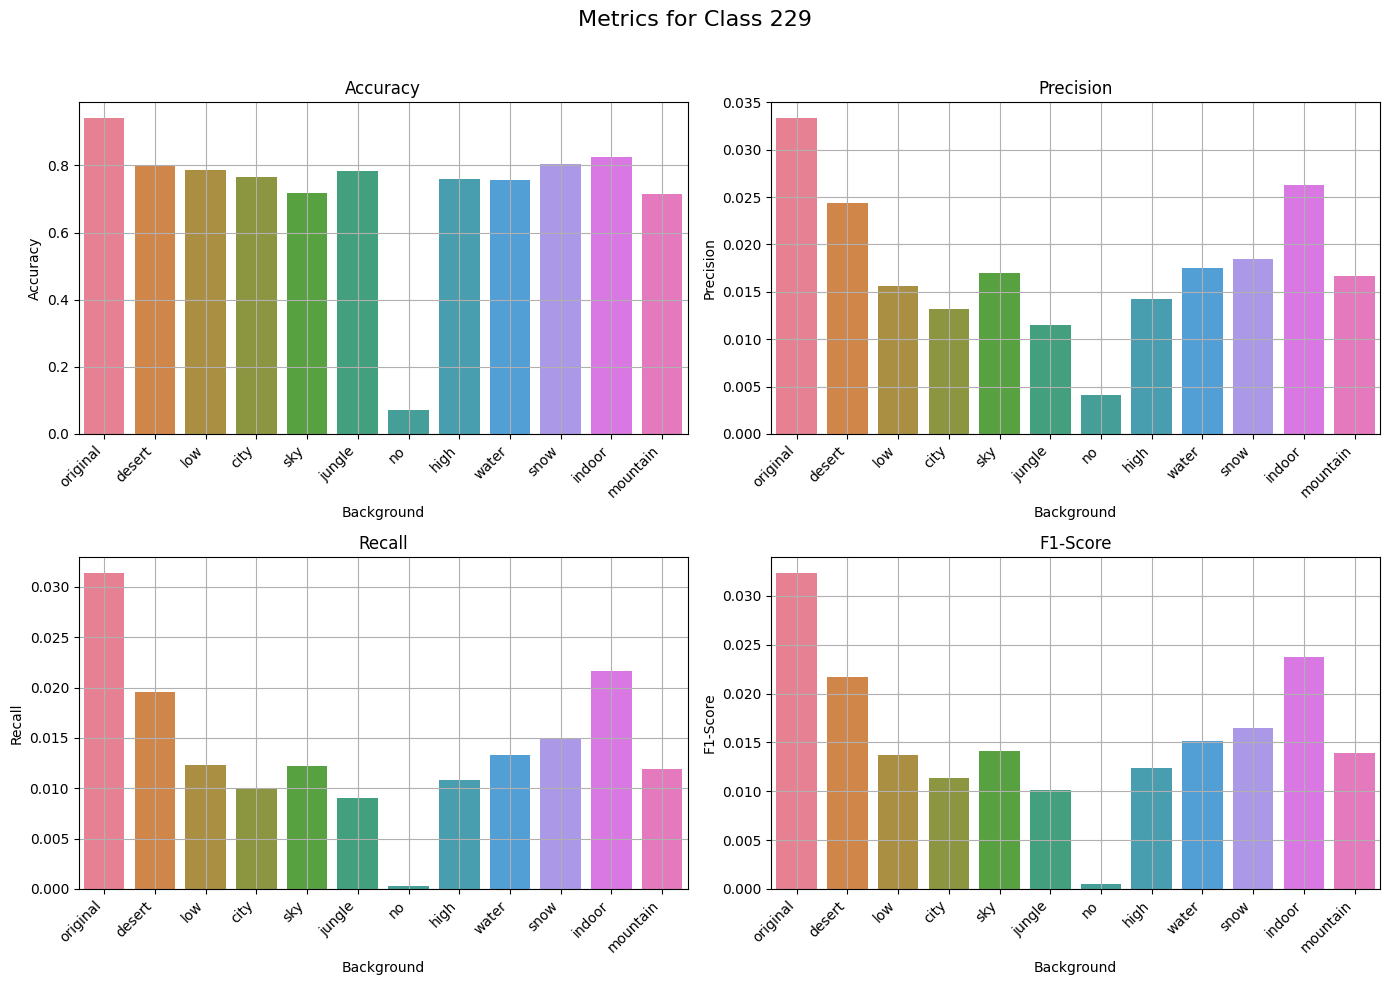
\includegraphics[width=.9\textwidth]{img/229}
	\caption{Metryki}
	\label{rys:229}
\end{figure}

\begin{figure}
	\centering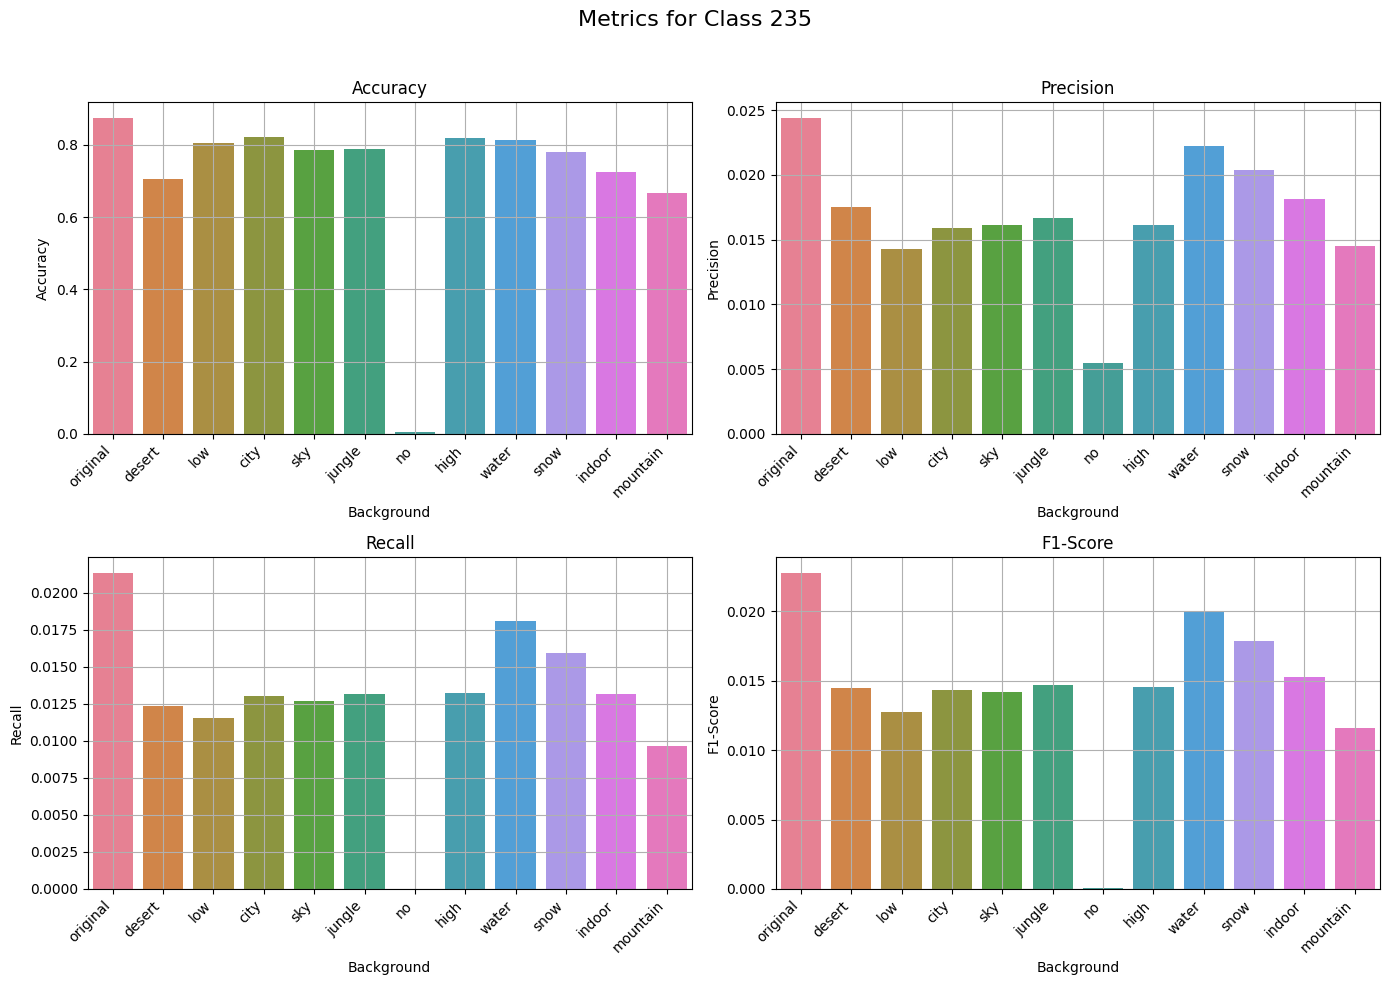
\includegraphics[width=.9\textwidth]{img/235}
	\caption{Metryki}
	\label{rys:235}
\end{figure}

\begin{figure}
	\centering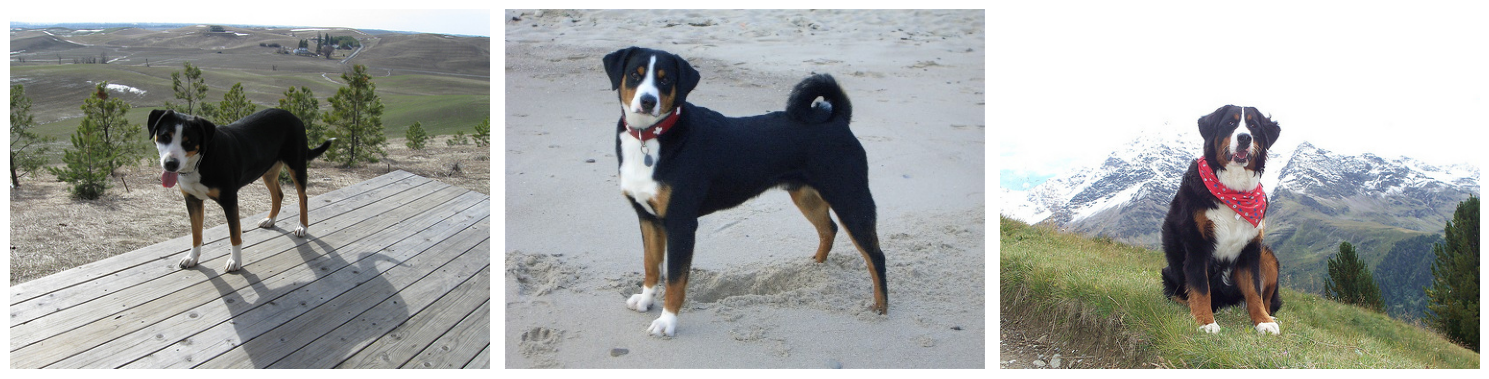
\includegraphics[width=.9\textwidth]{img/238}
	\caption{Metryki}
	\label{rys:238}
\end{figure}

\begin{figure}
	\centering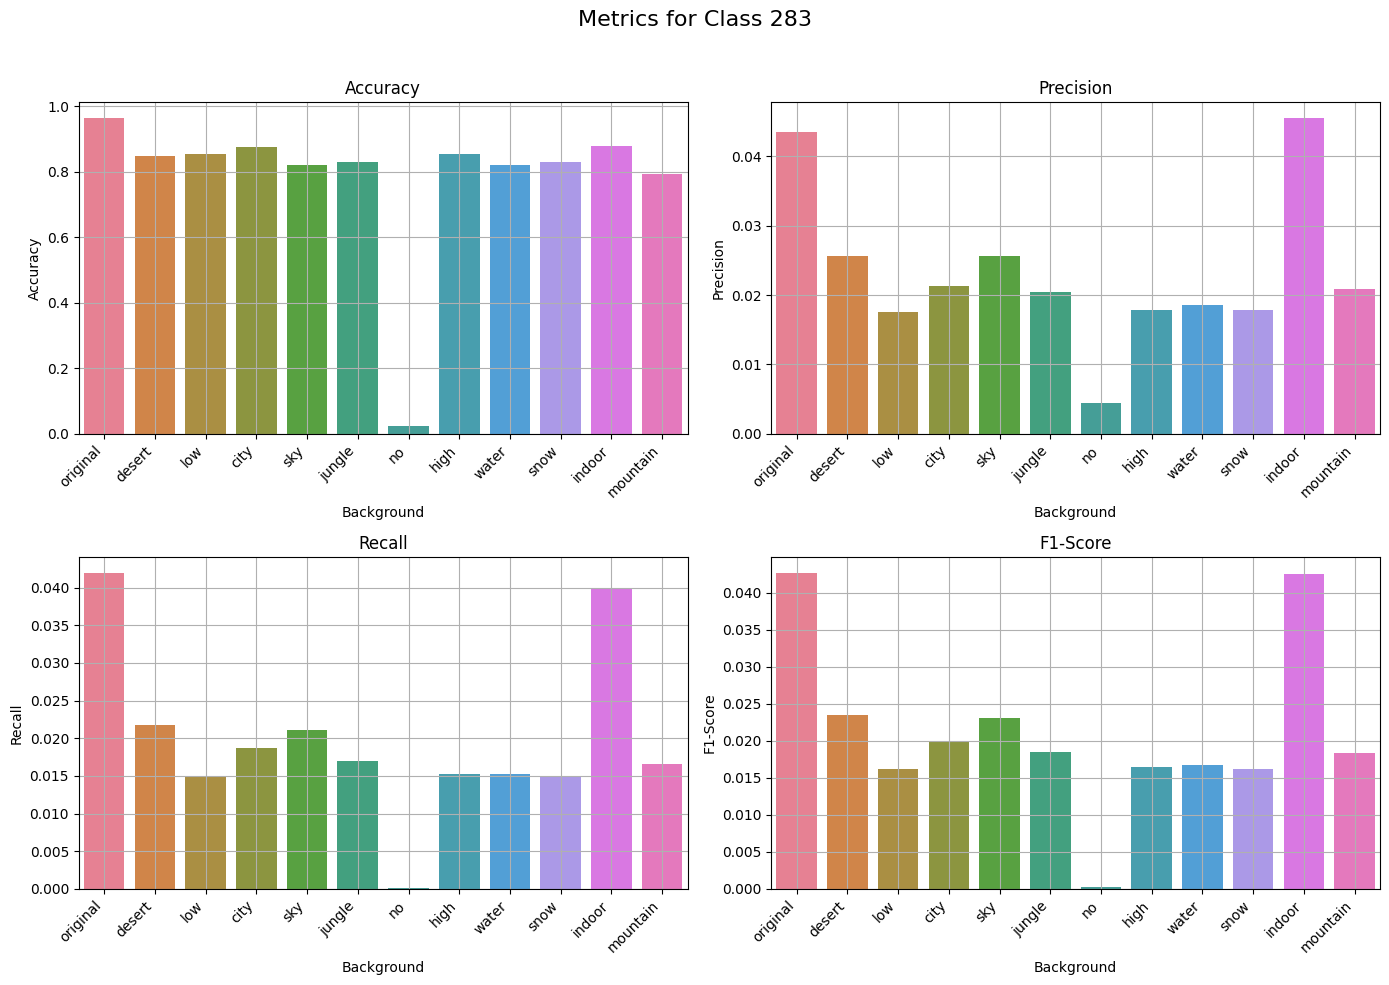
\includegraphics[width=.9\textwidth]{img/283}
	\caption{Metryki}
	\label{rys:283}
\end{figure}

\begin{figure}
	\centering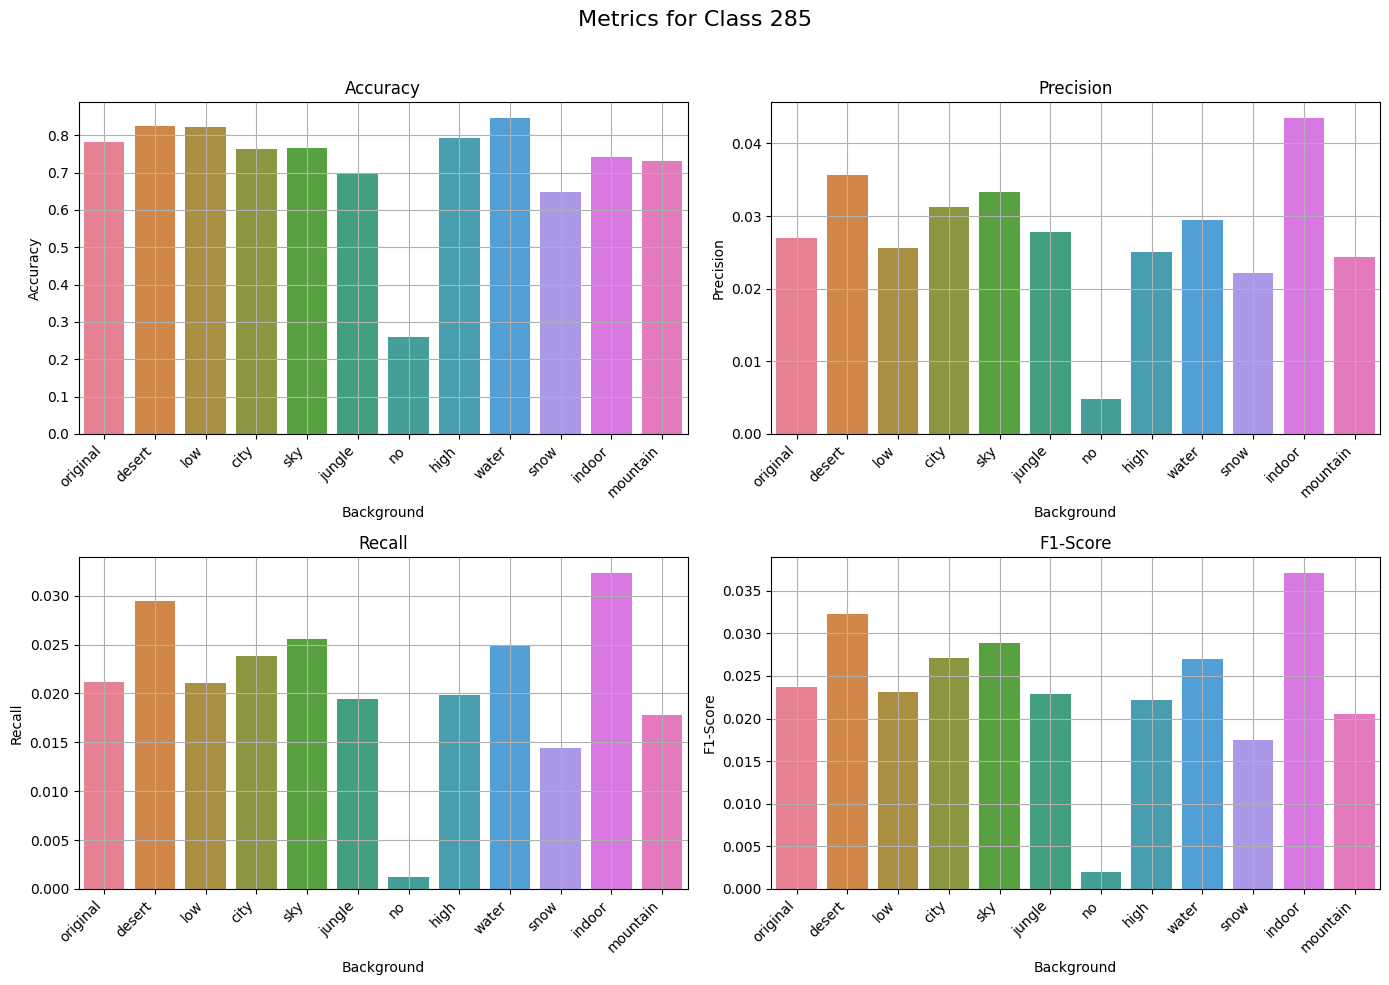
\includegraphics[width=.9\textwidth]{img/285}
	\caption{Metryki}
	\label{rys:285}
\end{figure}

\begin{figure}
	\centering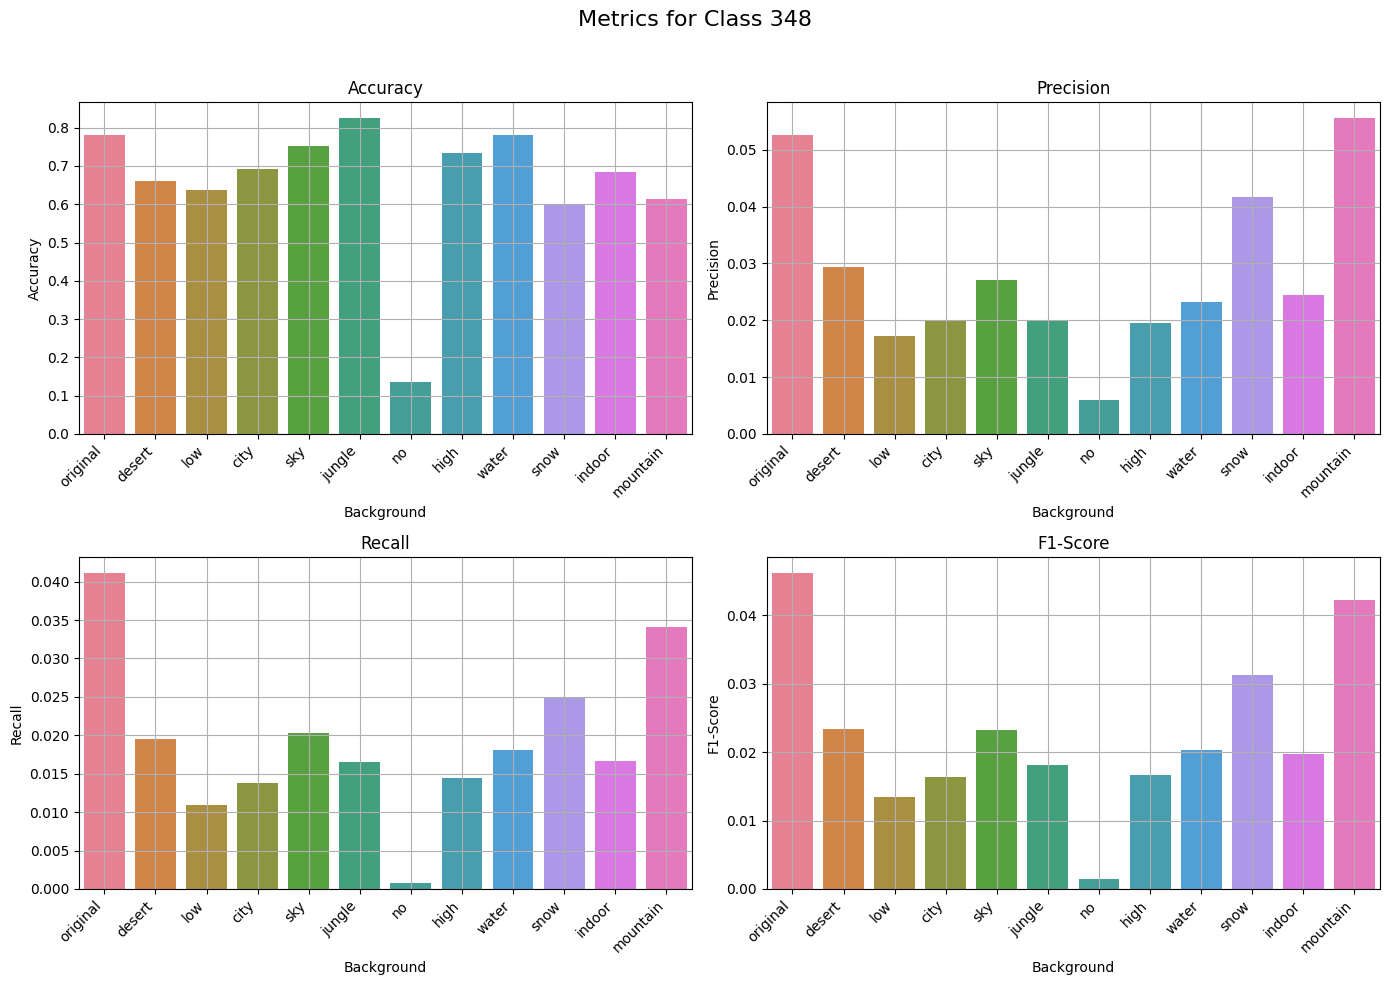
\includegraphics[width=.9\textwidth]{img/348}
	\caption{Metryki}
	\label{rys:348}
\end{figure}

\begin{figure}
	\centering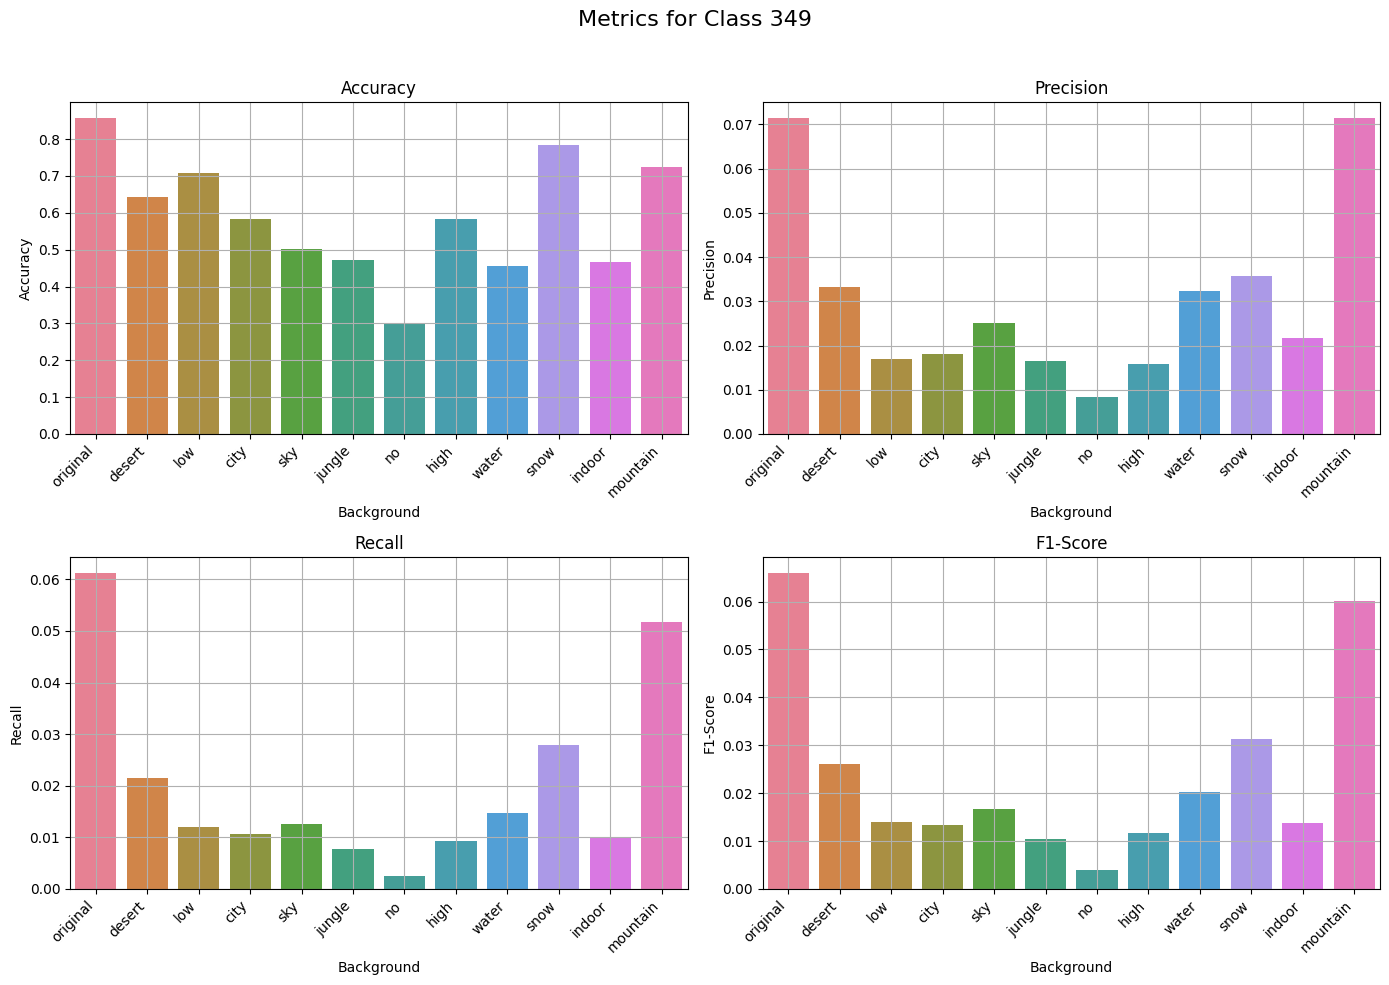
\includegraphics[width=.9\textwidth]{img/349}
	\caption{Metryki}
	\label{rys:349}
\end{figure}
